%\begin{savequote}[8cm]
%Alles Gescheite ist schon gedacht worden.\\
%Man muss nur versuchen, es noch einmal zu denken.

%All intelligent thoughts have already been thought;\\
%what is necessary is only to try to think them again.
%  \qauthor{--- Johann Wolfgang von Goethe \cite{von_goethe_wilhelm_1829}}
%\end{savequote}

\chapter{\label{ch:2-litreview}Background}

%\minitoc

 This chapter provides the necessary background for the topics of the thesis; first by summarising the main aspects of the tropical circulation and of the global monsoon and discussing the existing theories to explain the monsoon phenomena. Then, the American Monsoon System is introduced and detail is given on the Midsummer drought of southern Mexico and Central America and El Niño Southern Oscillation teleconnections to this monsoon. Finally, a summary of the literature on the role of stratospheric-tropospheric coupling in the tropics for monsoon variability is given. %the relevant background of the characteristics of American monsoon system and outstanding issues is given. 
\section{The tropical circulation and the global monsoon}\label{sq:bk_tropics}

Tropical climate is a result of the strong solar insolation received year-round that generally provides a stronger heating of the surface compared to extra-tropical latitudes. These latitudinal differences in insolation generate a meridional heat transport by the coupled atmosphere-ocean system. This means that the tropics have a positive annual net energy and the extra-tropics show a an annual negative net energy. 

The dynamics in the tropics is also distinct from extra-tropical latitudes due to other physical features such as the relative extent and location of the continents, the way in which gravity waves propagate throughout the atmosphere and a different impact of Earth's rotation upon the dynamics of parcels. 
Generally, tropical dynamics is considered to be less understood than mid-latitude dynamics, because most of the assumptions of mid-latitude dynamical frameworks break down in the tropics, but also because reliable data in the tropics was scarce until satelllites began providing continous reliable observations of the tropics in the 1980s \citep{emanuel2007quasi,webster2020dynamics}.
%Tropical climate is characterized  which cause evaporative fluxes. %which makes the tropics the warmest region of the planet. 


%This differential heating between the tropics and higher latitudes drives a meridional transport of energy by the ocean-atmosphere system.
%The strong incoming solar radiation warms the tropical oceans, which together with near-surface wind stresses produce large evaporative fluxes that create a very moist boundary layer and trigger deep convection.

 %he differential heating of land over ocean modulate the tropical circulation. % and ultimately convection. 
 Moist convection is arguably one of the characteristic traits of tropical climate as the dynamics and thermodynamic effects of deep moist convection has relevant feedbacks with the regional and large-scale circulation \citep{emanuel1994atmospheric,webster2020dynamics} and produces long-distance effects through propagating waves and anomalous circulations \citep{hartmann2015,li2018fundamentals}.
 Moist convective systems span different spatial and temporal scales, from short-lived cumulunimbus showers to tropical cyclones that can survive more than a week on the open ocean. Over sufficiently long scales, the mean deep moist convective activity also plays a significant role in determining the large-scale tropical circulation typically divided into meridional and zonal overturning circulations, the Hadley and Walker circulations.
 
The Hadley cell is the meridional overturning circulation that arises from the differential heating between the tropics and the midlatitudes. The Hadley cell is characterized by ascending motions in the tropics and descending motions in the subtropics, and acts to transport heat poleward from the equator \citep{lorenz1967}.  This Hadley cell migrates merdionally with the seasonal cycle, the winter and summer cells interact with each other but also with the midlatitudes through eddy momentum fluxes \citep{bordoni2008monsoons}. 
The Hadley cell is not zonally symmetric; the boreal summer Hadley cell, for instance,  is primarily a result of ascent in the Indian Ocean and the west Pacific regions with a minor contribution from ascending motions in Central and North America \citep{hoskins2020}. 

In spite of the fact that the large input of solar radiation is roughly uniformally distributed throughout the tropics on an annual mean average at the top of the atmosphere, the energy balance at the surface and the tropical circulation are not zonally symmetric. The prominent example of zonal asymmetry in the tropics is the Walker circulation. 
The Walker circulation is the zonal overturning circulation found in the equatorial Pacific Ocean characterized by ascending motion over the West Pacific and descending motions over the East Pacific\citep{walker1924,bjerknes1969,gill1980}. The dynamic and thermodynamic effects of the location and strength of convection associated with the Walker circulation have strong impacts across all the tropics and also the extratropics, known as teleconnections \citep{cai2019pantropical}.

 %The horizontal gradients of temperature in the tropical free troposphere are observed to be relatively small and when considered to be negligible allow to describe balanced dynamics framework in the tropics typically referred to as the weak temperature gradient (WTG) approximation \citep{sobel2001wtg}.


\begin{figure}[b!]
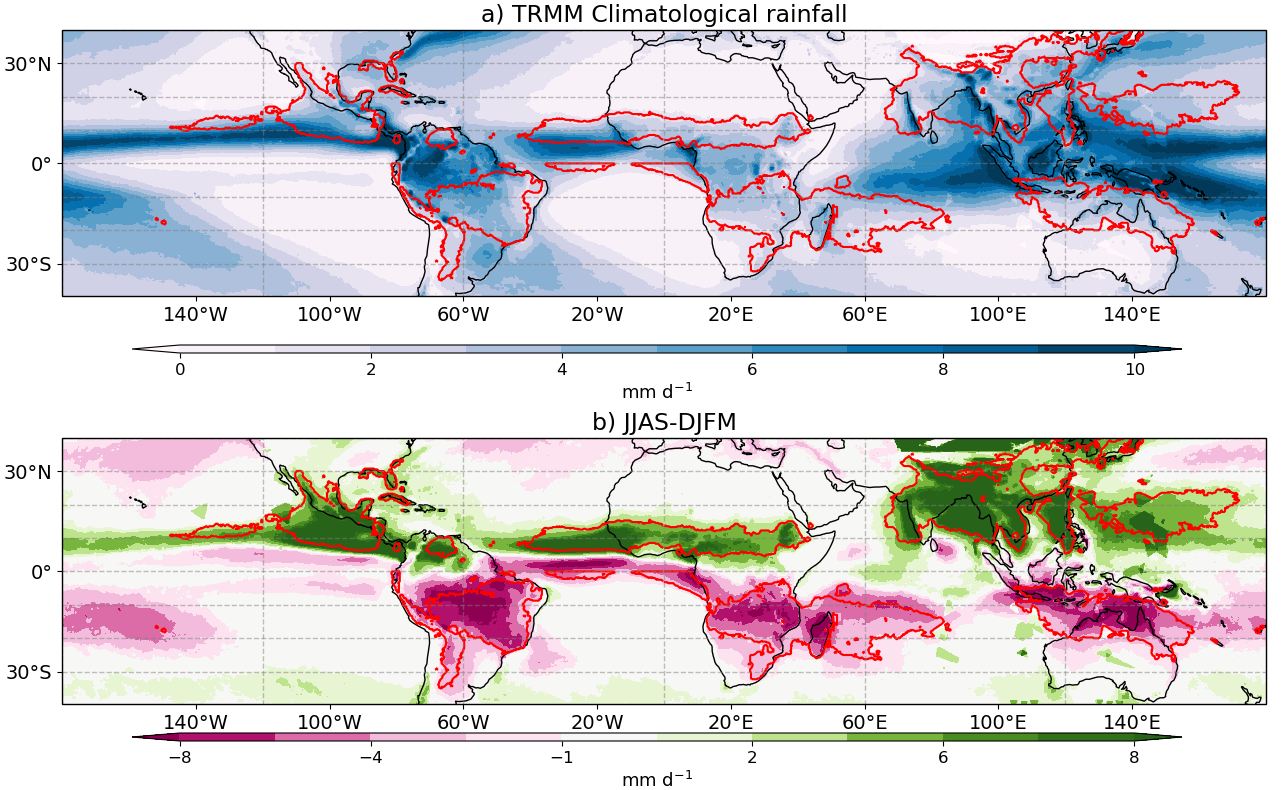
\includegraphics[width=\linewidth]{figures/trmmclima.png}
\caption{a) Climatological mean annual rainfall rates in the tropics using data from the Tropical Rainfall Measurement Mission (TRMM) dataset (1999-2018). b) The mean rainfall rate difference between boreal summer (JJAS) and austral summer (DJFM). The red contours highlight the regions where the mean summer rainfall amount accounts for more than 55\% of the mean total annual rainfall accumulation. }
\label{fig:monsoon}
\end{figure}

The Inter-tropical Convergence Zone (ITCZ) is a tropical band of convective clouds and precipitation that migrates meridionally with the seasons \citep{schneider2014}. The ITCZ is arguably one of the most relevant features of tropical climate due to the strong influence on the low- and upper-level circulation associated with ITCZ, the high tropospheric heating due to deep moist convection in the ITCZ and the largest precipitation rates in the tropics are found in the ITCZ.
The ITCZ is characterized by a strong convergent flow in the low levels and a strong divergent flow at upper levels. 
The meridional migration of the ITCZ, as well as the mean latitude of the ITCZ, results from the energy and momentum balances so that the ITCZ is predominantly north of the equator because of the inter-hemispheric temperature contrast \citep{donohoe2013,bischoff2016}.

One of the phenomena of tropical climate that first generated interest in climate research are monsoons \citep{halley}. The word \textit{monsoon} stems from the Arabic word for \textit{season} and is closely associated with the very first conceptions of a monsoon. 
The first widely accepted view of a monsoon was that of a large-scale land-sea breeze associated with the differential warming of the land and the ocean that force a seasonal reversal of the low-level wind flow that brought seasonal rainfall \citep{halley}. 

The traditional land-sea breeze definition of monsoon is now known to present several shortcomings. Firstly, several mid-latitude regions would fit a monsoon definition based solely on a seasonal reversal of the wind \citep{gadgil2018}, and secondly, regions that are now recognized as a monsoons, in South America for example, do not show a seasonal reversal of the winds, per se, rather just a seasonal change in direction and strength of the zonal winds \citep{vera2006}. For these reasons, the land-sea breeze view of monsoons has recently been replaced by three alternative conceptions, an ITCZ-monsoon framework, a convective quasi-equilibrium interpretation and a moist static energy (MSE) zonal-mean energetic interpretation \citep{biasutti2018global,hill2019,geen2020}. 
The MSE budget and methodology is detailed in section \ref{sq:msemethod} but a broad description of the method and summary of results arising from the MSE budget is given below.

The first framework  explains monsoons as a poleward extension of the ITCZ into land  generalizing all monsoons as an expression of global tropical convergence resulting from the energy balance \citep{chao2001origin,gadgil2018}. This interpretation has led to the concept of \textit{the global monsoon}, a term that encompasses all the regions in the tropics that exhibit a strong seasonality in precipitation \citep{zhou2016,gadgil2018}. 
In practice, the global monsoon refers to the those regions of the planet where more than 70\% of the total annual rainfall falls during the summer season, in several recognizing the seasonality of precipitation as the key feature to diagnose a monsoon \citep{zhou2016,wang2017}.

Figure \ref{fig:monsoon} shows the global monsoon as depicted by the TRMM dataset. By this definition, the majority of the regions over land between 5 and 10 degrees away from the equator are part of the global monsoon.
A regional monsoon, such as the Indian Monsoon, is then a subset of the global monsoon with unique regional characteristics that shape this monsoon different to other regional monsoons in terms of the seasonality, the strength and the dynamics. 
The American Monsoon System is then the regional monsoon that is located in the subtropics of North and South America. 


\cite{bordoni2008monsoons} provide an alternative conceptual view of monsoons, describing the characteristic rapid onset of a monsoon as a regime transition of the Hadley cell from a edddy-momentum  driven circulation, which resembles a canonical ITCZ regime, to a thermally direct circulation which resembles a monsoon-like circulation. The zonal mean MSE meridional gradient drives the ITCZ location and determines the strength of the overturning circulation by modulating the ventilation from midlatitude cooler and drier air in a feedback mechanism \citep{geen2020}. Even though this framework is posited as an axisymmetric framework, their predictions were broadly consistent with the Asian monsoon circulation. 


Convective quasi-equilibrium (CQE) is a theory for moist convection where convection sets the vertical temperature and moisture profiles to a convectively neutral state, thereby setting the free tropospheric temperature \citep{neelin2007moist}. For a monsoonal circulation, this theory emphasizes the coupling of convection and dynamics predicting that the subcloud layer equivalent potential temperature maxima must be collocated with the free tropospheric saturation equivalent potential temperature \citep{nie2010observational,geen2020}. The rapid onset of the Asian monsoon has been shown to be associated with the boundary layer moist entropy distribution, in agreement with predictions of CQE \citep{nie2010observational,boos2015review,ma2019}.

Several studies examine the monsoon phenomena through an axi-symmetric framework that assummes zonal symmetry and aims to understand the large-scale dynamical influence over the extent and strength of the axi-symmetric monsoon through global energetic diagnostics \citep[e.g.][]{faulk2017effects,geen2019,byrne2020}. The zonal-mean framework is common to the Hadley cell interpretation of monsoons \citep{bordoni2008monsoons}, as well as the ITCZ-monsoon theory. %This framework is very much in line with the global monsoon concept, that implies a zonally symmetric circulation driven by global energetic balance. 
However, regional monsoons are shaped by the asymmetries imposed by the orography, the characteristics of the surrounding ocean basins, land-sea contrasts and also the role of vegetation-hydrology coupling \citep{wang2017,pascale2019}. 
The importance of zonal asymmetries has raised multiple issues with large-scale so-called monsoon dynamics theories, as several predictions of these theories are not consistent with observations of regional monsoons \citep[e.g.][]{nie2010observational,smyth2018simulated,biasutti2018global,pascale2019}. 


Recent reviews acknowledge that all these frameworks have significant shortcomings to be applied to regional local monsoons \citep{biasutti2018global,hill2019,geen2020}. These reviews conclude that a framework that reconciles the global energetic perspective with the characteristics of regional monsoons would be crucially important and very useful, but as several authors point out \citep[e.g.][]{biasutti2018global,hill2019}, also very hard to formulate. For example, the North and South American Monsoons depart from CQE, as precipitation does not follow the maxima in subcloud equivalent potential temperature \citep{nie2010observational,geen2020}. 

 The MSE budget framework suffers both from theoretical and practical shortcomings. One practical shortcoming is that the calculation of the budget terms post hoc in reanalysis or models results in very large residuals \citep{hill2019}, so these frameworks work best when the calculations are done inside the budget terms to be integrated online at each time-step \citep[e.g.][]{ma2019}.
The theoretical shortcoming is that the surface fluxes over land, e.g., in the Sonoran and Saharan deserts and the deep Amazon make the estimations of the roles of hydrology-vegetation feedbacks and their potential contributions to the MSE budget in observations very difficult to assess \citep{boos2016,pascale2019}. The use of simpler moisture budgets has proven useful in a regional monsoon context to investigate the sources of moisture for a monsoon in current  \citep{ordonez2019,martinez2019} and future climates \citep{smyth2020}, but this budget is mostly a tool and not a coherent theory for process-level understanding of monsoons.

 
The Hadley cell interpretation of monsoons has significant shortcomings to depict some regional monsoons, particularly those that are not the Asian monsoon as the overturning circulation in the South Asian monsoon is strong enough to be represented by a clear thermally direct regime.
However, this energetic framework assumes no zonal transport of energy, which minimizes the role of orography and land-sea interaction \citep{biasutti2018global}.
One might reasonably infer from these results that the timing of transition in zonal mean overturning cells would be similar for monsoons at different longitudes but similar latitudes, which is not the case \citep{wang2017}.
Furthermore, a monsoon restricted to a small area, such as a the North American and African monsoons may not present a clear zonally averaged overturning regime, and may be significantly affeced by local zonal shallow and deep circulations \citep{zhai2015regime}. For instance, \cite{smyth2018simulated} shows that the simulated West African monsoon when forced with different solar forcings exhibits a decoupling between the zonal-mean ITCZ location, the strength of the local Hadley cell and the monsoon rainfall, in opposition to the predictions of this framework \citep{bordoni2008monsoons}.


In short, despite significant progress in our understanding of the monsoon phenomena a the planetary-scale through zonal mean energetic frameworks, there is an important gap between large-scale theories of monsoon dynamics and the observed regional monsoons. 
The next section presents a summary of the American Monsoon literature, which explains the characteristics of these monsoons through the effect of regional features and dynamics, seemingly detached from the literature in this section. The AMS literature is therefore, seemingly, detached from the literature in this section.

\section{The American Monsoon System}\label{sq:bk_ams}

\begin{figure}[t!]
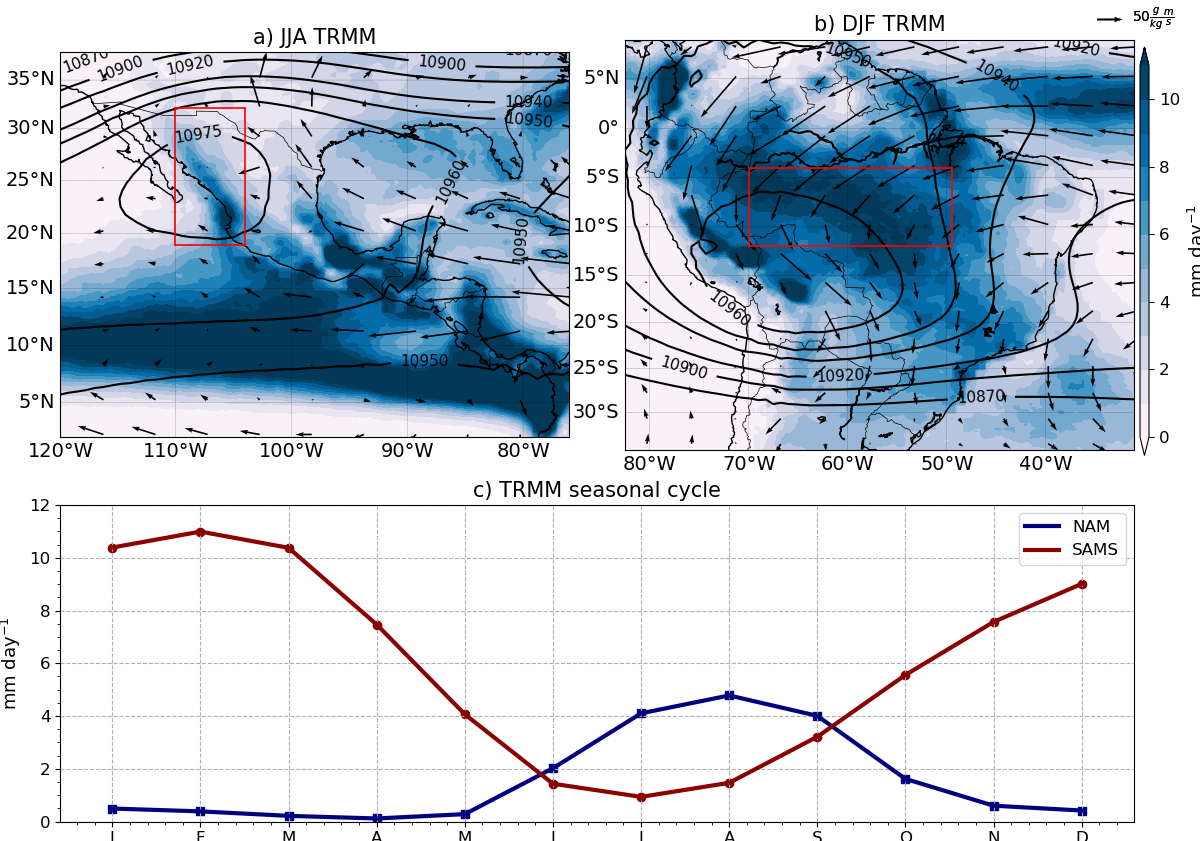
\includegraphics[width=\linewidth]{figures/amsclim.png}
\caption{ Climatological mean a) boreal and b) austral summer rainfall (shading), 850 hPa moisture flux (vectors) and geopotential height at 250 hPa (contours) in a) southern North America and b) South America. c) Monthly-mean seasonal march of precipitation in the TRMM dataset for two area-averaged time-series, the North American Monsoon (NAM) and the South American Monsoon System (SAMS) shown in the red rectangles in a-b). }
\label{fig:americanmonsoon}
\end{figure}

The American Monsoon System (AMS) is the main source of rainfall for tropical Latin America and is typically subdivided into the North and South American monsoon systems \citep{vera2006}. 
Although the spatial definition of the AMS is quite varied amongst studies, a general consensus is that the North American Monsoon is found in south-western North America (Figure \ref{fig:americanmonsoon}a) extending north from central-west Mexico into the southwestern United States and the South American Monsoon is centred in the deep Amazon south to the river mouth (Figure \ref{fig:americanmonsoon}b) \citep{adams1997,stensrud1997,vera2006}.


 The seasonal cycle of rainfall in the North American Monsoon is characterised by a wet July-August-September season and significantly drier conditions during the rest of the year \citep{adams1997} (Figure \ref{fig:americanmonsoon}c).
Three temporal stages describe the evolution of the North American Monsoon \citep{adams1997,geil2013}.
First, the onset stage (May-June) starts with a strong surface warming that leads to very high temperatures in the desert region.
Simultaneously, the sub-tropical jet weakens and migrates north decreasing the frequency of mid-latitude disturbances in the monsoon region \citep{douglas1993,turrent2009}.
These factors combine to develop a low-level (upper-level) thermal surface low (anticyclone) and  moisture influx from the nearby Gulf of California and easternmost Pacific Ocean \citep{douglas1993,geil2013}.
Maturity (July-August) is the peak period of monsoon rainfall characterised by sustained deep convection \citep{barlow1998} and significant increases in low and mid-level moisture flux convergence and mid-level latent heating \citep{adams1997,cook2013}. This latent heating caused by deep convection can be diagnosed in the upper-level geopotential height (Figure \ref{fig:americanmonsoon}a) in the form of an anticyclone centred on the monsoon region. 

The moisture flux convergence decreases in August, after which precipitation recycling \citep{dominguez2008} plays an important role in keeping deep convection active until September.
 Decay (September-October) is the last stage of the monsoon, in many ways opposite to the onset stage, as is characterised by the equatorward migration of the sub-tropical jet \citep{higgins1997,geil2013}, evaporation in the nearby basins decreases and deep convection in the monsoon region gradually disappears \citep{douglas1993}.

 The origin of the high levels of moisture at low and midlevels in the monsoon region has been a matter of debate for a long time \citep{adams1997,barlow1998,vera2006,ordonez2019}.
A large number of studies aknowledge that the main source of moisture for the North American Monsoon is the East Pacific Ocean and to a second order, mid-level moisture advected from the Gulf of California can mix in the column \citep[e.g.][]{adams1997,stensrud1997,vera2006,turrent2009,ordonez2019}.
 %The high specific humidity in the mid-troposphere has been explained as the product of deep convection taking place on advected parcels from the EPO and GoC in combination with moisture mixing from the Gulf of Mexico \citep{douglas1993,stensrud1997,turrent2009}.

%A key aspect of this monsoon is the moisture advected by the low-level flow from the Gulf of California and the East Pacific Ocean and to a lesser extent the moisture mixed in the mid-troposphere from the Caribbean Sea and Gulf of Mexico \citep[e.g][]{stensrud1997,pascale2016,ordonez2019}.

The South American Monsoon is a primary source of precipitation for South America, especially in the Amazon region \citep{gan2004,vera2006,jones2013}.
During austral summer (DJF), monsoon rainfall accounts for over 60\% of the total annual precipitation in the Amazon \citep{gan2004,marengo2012}, whereas
austral winter rainfall accounts for less than 5\% of the total annual rainfall \citep{vera2006}.
In the central Amazon, convective precipitation is observed from early October but the main rainy season extends from December to April \citep{machado2004,adams2013}, whereas convection in southeastern Brazil and Paraguay starts in November and peaks in January and February \citep{marengo2001,nieto2011}. 

A surface heat low appears in Bolivia in early austral summer, known as El Chaco Low, as a result of strong warming in austral spring \citep{marengo2012,sulca2018}.
 As this surface heat-low strenghens, low-level convergence drives the circulation into the low region.
 Simultaneously, an upper-level anti-cyclone (Fig. \ref{fig:americanmonsoon}b), known as the Bolivian High, develops in the same region as a signature of strong deep convection and latent heating \citep{marengo2001,vera2006}.

This low-level wind circulation importing moisture from the Atlantic is one of the most important features of the SAMS \citep{marengo2012,wang2017} as the flow modulates the moisture flux to the mainland and influences the ocurrence of active and break phases of the SAMS \citep{jones2002}, as well as changes in the temporal and spatial
distribution of rainfall \citep[e.g.][]{giannini2004,bombardi2011}.

As described in the previous sections, both the North and South American monsoon thermodynamics do not follow the CQE propositions, i.e., the maximum low-level moist static energy is not collocated with the maximum free tropospheric temperature. 
One possible reason for this is that the free-troposphere over southwestern North America is significantly drier than in other monsoon regions, decoupling the free troposphere from the boundary layer. One alternative hypothesis is that ventilation of low moist entropy air from the midlatitudes is responsible for this decoupling of the boundary layer and the free troposphere in the American monsoons \citep{boos2015review}.

%The SAMS and NAM did not fit the tradditional view of monsoons as the seasonal reversal of the winds was not as strong and clear as for other monsoons such as the Indian monsoon \citep{}. However, there is seasonal contrast in the zonal winds in both the NAM and SAMs as composite DJF-JJA wind differences suggest. 
%Furthermore, the NAM lower-level temperature structure departs from the quasi-equilibrium framework. A monsoon, can be described, through quasi-equilibrium arguments, \citep{}. %structures

\section{A review on the proposed mechanisms for the Midsummer drought}\label{sq:litmsd}


The characteristics of the seasonal cycle of precipitation in northwestern Central America, the Caribbean and southern Mexico fit the definition of a monsoon climate \citep{wang2017} with a clear separation of the wet and dry seasons. 
However, this region shows a unique climatological precipitation feature. After monsoon onset, rainfall decreases considerably around the midsummer; this decrease is followed by a secondary increase in precipitation in the late summer \citep{mosino1966}, and for this reason this feature of the seasonal cycle is most commonly referred to in the literature as Midsummer drought (MSD) \citep{magana1999}.   


The intraseasonal variations of precipitation associated with the MSD have been known for centuries and have shaped agricultural practices in the region. 
For example,  ancient mayan texts suggest that agricultural rituals associated with the plea for rain-bearing clouds to the gods were significatnly more frequent during the drier MSD period \citep{jobbova2018ritual}. In current days, the MSD is well known by local farmers who refer to the drier midsummer period as `El Veranillo' in Central America and `can\' icula' in southern Mexico because the drier period  coincides with the Canis Major constellation appearing in the sky \citep{dilley1996}.
% so that the MSD variations have shaped agricultural practices in the region for centuries.
%
% Save paragraph for onset method! 
%Farmers in Central America who are subject to climatic stress due to droughts, have already perceived and adapted to changes in the characteristics of the rainy season, such as the timing and strength of the midsummer drought \citep{hellin2017,de2018,harvey2018}, but it is unclear whether these perceived changes are a real trend in the observations \citep{anderson2019multiscale}. 

The two peak structure of the MSD has been diagnosed in the observed climatological precipitation of several regions of Mexico, El Salvador, Belize, Guatemala, Costa Rica and Cuba \citep[e.g.][]{mosino1966,magana1999,duranquesada2017,perdigon2018,martinez2019}.
However, notable differences in the seasonal cycle of precipitation have been found between the mainland Central America and the Caribbean islands. The so-called first peak of precipitation occurs in June and the second peak in September in northern Central America whereas the two peaks are observed in May and October in the Caribbean.

%The mechanisms that cause the MSD have been debated since the first observational descriptions of the phenomenon \citep[e.g.][]{mosino1966}, as studies that aimed to explain the physical mechanisms MSD have not yet reached a consensus.
 In spite of extensive research to understand the physical mechanisms associated with the MSD   \citep[e.g.][]{magana1999,giannini2000,gamble2008,herrera2015,maldonado2017,straffon2019}, debate remains over which is the leading-order mechanism that causes rainfall to decrease at midsummer and increase again at the end of the summer.  % why rainfall increases again at the end of the summer, the end of the MSD, and why this happens at this time of the year. 
%Dynamical or thermodynamical mechanisms have been put forth and different roles have been proposed for the Atlantic and the East Pacific Oceans \citep[e.g.][]{magana2005,gamble2008,herrera2015}. 
Fundamental questions remain unclear such  as whether the MSD is caused by two precipitation enhancing mechanisms \citep{karnauskas2013} or a mechanism that inhibits rainfall at midsummer \citep{duranquesada2017}. 
Furthermore, the association between the MSD in Central America and in the Caribbean is still disputed \citep{gamble2008}, as most studies suggest that the two regimes are unrelated and therefore two different explanations are required to account for the two MSDs in these regions. 

%Any complete theory or conceptual model must account for the following characteristics of the seasonal cycle. First, the theory must explain the timing and strength of the first peak of rainfall. Second, the timing and strength of the MSD, i.e., what causes rainfall to decrease at midsummer. Finally, the theory must explain the timing and mechanism driving the second increase in precipitation after the midsummer. %The lack of a clear understanding of the processes that modulate the MSD makes climate change projections uncertain. 

One of the first hypotheses to account for the bi-modal distribution of rainfall was proposed by \cite{hastenrath1967} who argue that a double crossing of the ITCZ can explain the MSD so that the first peak of precipitation is associated with early summer northward crossing of the ITCZ and the second peak the return or southward displacement of the ITCZ during late summer.
However, this theory fails to explain the MSD signal seen at latitudes as high as 29$^\circ$N \citep{perdigon2018,zhao2020}, a feature that will be shown in this thesis, which is further north than the northernmost extension of the ITCZ \citep{schneider2014}, and certainly the ITCZ does not cross twice so far from the equator. % \citep{magana1999,magana2005}.

\cite{magana1999} and \cite{magana2005} proposed a mechanism driven by radiative-convective feedbacks between the East Pacific (EP) sea-surface temperatures (SSTs) and deep tropical convective clouds. The coupling between the height and strength of convection, the incoming shortwave radiation and the SSTs are the key features of their framework. %Convection feedbacks with SSTs evaporation and
%moisture flux into the MSD region. 
The EP SSTs peak in May triggering large evaporative fluxes and deep convection in the EP ITCZ and the western coast of Central America.
The high convective clouds produce a radiative cooling effect at the surface due to a decreased incoming shortwave radiation associated with the reflectance of shortwave radiation by clouds.
This cooling  decreases SSTs and deep convective activity and thus accounts for the decrease of rainfall during the midsummer.
The second peak in September is driven by an opposite mechanism, i.e., the decreased frequency of deep convective clouds during the MSD period in July and August reduce the cooling effect of the anvil clouds and increase the incoming shortwave radiation at the surface, SSTs and surface fluxes, all of which leads to an precipitation during late August and September \citep{magana1999}.


%have been linked to several sources of seasonal variability,
%but debate is far from uncontroversial as to which is the principal mechanism to account for the MSD.
A large number of studies, in contrast, propose that the seasonal evolution of the North Atlantic Subtropical High (NASH) is the leading mechanism for the MSD \citep[e.g.][]{mapes2005,small2007,gamble2008,curtis2008,munoz2008,martinez2019,corrales2020}. The NASH is the subtropical anticyclone in the North Atlantic Ocean that migrates southwest during early boreal summer. The expansion and intensification of the NASH in boreal summer, according to these studies, strengthens the low-level trade winds, controlling the seasonal cycle of a low-level jet found in the core of the Caribbean Sea known as the Caribbean Low-Level Jet (CLLJ). The CLLJ is a key regional feature of the climate of the Caribbean and the Intra-Americas Sea  because the strength and direction of the flow in the Caribbean controls the underlying Caribbean SSTs and the regional moisture transport \citep{giannini2000,mestas2007,martinez2019,garcia2020sub}. 

% which then influences the low-level wind flow over the western coast of the continent, in the easternmost Pacific Ocean.
 
 
 However, studies disagree on the specific roles that the CLLJ and the NASH play for the precipitation over the Mesoamerican region. 
 For example, some studies \citep[e.g.][]{giannini2000,mestas2007,gamble2008} suggest that  the expansion of the western flank of the NASH strengthens the CLLJ which cools the SSTs, through the effect of wind stress and mixed-layer mixing.
The cooling of SSTs diminishes evaporation and therefore low-level moisture which ultimately leads to less precipitation. 

In contrast, other studies propose that the CLLJ and NASH affect the seasonal cycle of precipitation through their effects on the regional moisture transport \citep{small2007,munoz2008,herrera2015,duranquesada2017,martinez2019}. In this second hypothesis, the changes to the intensity of CLLJ influenced by the NASH modify the convergence and divergence patterns in the Intra-Americas Sea. In other words, the midsummer strengthening of the CLLJ increases moisture divergence, drying the atmospheric column over the Caribbean. 


%GCM literature needed.
 
    
%The strength of the easterlies crossing from the Caribbean Sea to the EP Ocean has been argued to modulate ascending and descending motions all across the Intra-Americas Seas region through the  effects of vertical wind shear and moisture divergence  \citep{herrera2015,corrales2020,zhao2020}. Moisture budgets over the Caribbean have diagnosed that changes to the regional and temporal distribution of moisture \citep{duranquesada2017,martinez2019,martinez2020} can influence the intra-seasonal and inter-annual variability of precipitation. % can be explained by the variability of the easterly wind flow in the CLLJ and the EP Ocean \citep{herrera2015,martinez2019,zhao2020}. 


%The strength of the flow crossing  between the EP Ocean and the Caribbean Sea has been argued to be a a function of the SST gradient across the basins, at least on interannual time-scales \citep{martinez2020}. This is particularly relevant as the Pacific Ocean is projected to warm more than the Caribbean Sea in future decades, which could change the SST gradient, strengthen the CLLJ and shift the regional precipitation patterns \citep{corrales2020}.
    
 \cite{herrera2015} shows that during the drier months in Central America in the Midsummer, convective west of the central American continent gets stronger with heavier precipitation.  Their evidence suggests that the gap flow that originated from the CLLJ in the Caribbean Sea controls the location of ascending and descending motions, and the MSD may be explained by the seasonal variations and the coupling of the low-level wind flow with the underlying EP SSTs.
\cite{herrera2015} further argued that the exit region of the CLLJ is located to the east of the region of strongest MSD signal, which suggests that the moisture divergence effect over the central American MSD is minimal. 



A different mechanism, proposed by \cite{karnauskas2013}, argues that the biannual crossing of the solar declination angle can control precipitation and explains the bimodal characteristics of the seasonal cycle. In this mechanism, the MSD is driven by two precipitation enhancing periods that are separated by a relatively normal, and drier, period. This theory differs from those previously discussed which explained the MSD through mechanisms that inhibit convective activity in the midsummer whereas \cite{karnauskas2013} argues that the solar declination angle that crosses twice through Central America, once during June and a second time during September, increases convective activity during each crossing. 

The variations of incoming shortwave radiation associated with the declination angle modulate the SSTs, surface fluxes and therefore convective activity. In other words, the first crossing of the solar declination angle increases the incoming shortwave radiation which increases the SSTs, evaporation and leads to a peak of precipitation, i.e., the first peak. After the shortwave radiation is reduced the MSD period appears. The second crossing of the solar declination angle, similarly, explains the second peak as the second increase in incoming shortwave promotes more deep convection than during the MSD. 



Other mechanisms have been proposed arguing that the MSD is a result of vertical wind shear affecting convective instability or the Saharan dust controlling  the microphysics of clouds \citep{angeles2010origins}.
For instance, \cite{perdigon2019} also finds a link between the frequency and spatial distribution of the first peak rainfall rates and the Madden-Julian Oscillation. 

\section{El Niño Southern Oscillation: impacts to the American monsoon system}
\label{sub:lit_enso}



 El Niño-Southern Oscillation (ENSO) is a phenomena that primarily affects the local ocean and atmosphere of the equatorial Pacific Ocean, but these changes are profoundly important for the global climate system, which is why ENSO is commonly known as the leading mode of interannual variability. 
 The term \textit{'El Niño'} was initially coined by Spanish colonizers when they learnt from Peruvian fishermen that the ocean surface temperatures in the easternmonst Pacific Ocean increased notably in some years around December time. 
 For religious reasons, the colonizers termed the SST increase as Christ Child -- \textit{El Niño}. 
 %The effect teleconnections can be felt in the tropics through changes in the tropical overturning circulation but also impacting extratropical circulations and thus ENSO impacts extend to most regions on the planet.
 
 
 
  Later on, sir Gilbert \cite{walker1924} coined the term \textit{Southern Oscillation} to describe the synchronous changes to the sea-level pressure of the Indo-Pacific region and South America. 
  \cite{walker1924} and \cite{walker1932} are the first analyses of synchronous effects of the tropical circulation over local precipitation, temperature and pressure. Further research \citep[e.g.][]{troup1965} would highlight that these remote changes in pressure were driven by the east-west pressure gradient in the equatorial Pacific. 
  
  The changes in the pressure field associated with the Southern Oscillation (SO) are now part of what is known as the Walker circulation, which intertwines the dynamics of the zonal circulation in the East Pacific with the SSTs over the underlying ocean. ENSO is then characterized as a coupled phenomena composed of an oceanic part, \textit{El Niño}, and an atmospheric component associated with the zonal circulation but best characterized by changes to the surface pressure field, the Southern Oscillation. 
  
  
% The SO changes are intertwined with changes to the Walker circulation as the surface pressure variations affect the strength of low-level trade winds, which are a big component of the Walker circulation. In other words,   ENSO is the coupled ocean-atmosphere oscillation of the equatorial Pacific sea-surface temperatures (SSTs) and the atmospheric pressure and wind fields, particularly those associated with the Walker circulation\citep{wang2004}. %; these variations in the SO are typically described as with the Walker circulation. %changes and the Southern Oscillation (SO) is associated with changes in the zonal gradient of MSLP. Combined, El Niño and the SO compose the ENSO phenomenon.
  
\begin{figure}[t!]
\centering
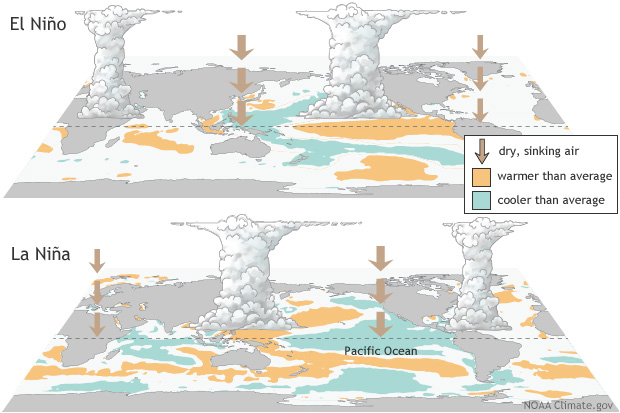
\includegraphics[width=\linewidth]{figures/ENSO}
\caption{Schematic of the positive (upper) and negative (lower) phases of ENSO. Regions with tall clouds indicate more ascent and convection than normal whereas brown arrrows indicate dry descending air. Obtained from the National Oceanic and Atmospheric Administration at \url{https://www.climate.gov/enso}. }
\label{fig:enso}
\end{figure}  
 ENSO has several unique features, such as no robust periodicity as events may occur every 2 to 7 years and a seasonal phase-locking that are associated with ENSO events peaking in boreal winter in observations \citep{wang2004}. Even though the underlying physics that cause ENSO and explain the variability in the periodicity of the phenomena is still debated \citep{wang2004,christensen2017}, several aspects are now better understood. 
For example, the local effect that ENSO events have over on the location and strength of deep convection in the equatorial Pacific have long been thoroughly described \citep{trenberth1997,neelin1998}. 

During a neutral state of ENSO, the Walker circulation is found in the climatological state, with ascent and wet conditions in the West Pacific  and descent and drier conditions in the East Pacific. During El Niño the Walker circulation and low-level trade winds weaken which is associated with an eastward shift of deep convection along the equatorial Pacific (Figure \ref{fig:enso}), with convective rainfall becoming more frequent in the central and even eastern Pacific than normal \citep{neelin1998,wang2004}. During La Niña the opposite happens and the Walker circulation stregnthens which leads to stronger convection in the West Pacific and stronger ascent on the East Pacific (Figure \ref{fig:enso}). 


In other words, ENSO imposes a strong control on the location and strength of the Walker circulation (Figure \ref{fig:enso}). These changes to the strength and position of the convective regions in the Pacific Ocean can then propagate to other regions of the planet; these far-distant effects are commonly known as \textit{teleconnections}.  
For example, ENSO has a direct effect over other tropical regions outside of the Pacific through the Walker circulation, see Figure \ref{fig:enso}, as upper-level wind anomalies induce anomalous vertical motions over the monsoons in West Africa \citep{ropelewski1986,ropelewski1987} or South America \citep{sulca2018}.  
  Other mechanisms of ENSO teleconnections to higher latitudes include changes to the position and strength of sub-tropical jets \citep{fereday2020}, changes to the Pacific and North American circulation patterns \citep{bayr2019} as well as impacts to the North Atlantic via the stratospheric polar vortex \citep{domeisen2019}.
  
  In South America, the effects of ENSO are felt throughout the continent and throughout economic sectors from Peruvian fishermen \citep{takahashi2004} to the Amazon rain-forest and the plainlands in South-eastern South America\citep{grimm2011,marengo2012}. 
  One key aspect of current research on ENSO impacts to South America is the observed non-linearity and non-symmetry in the teleconnections, which has mainly been attributed to ENSO diversity \citep{tedeschi2015,cai2020}.
A non-linear teleconnection refers to a non-linear scaling between the strength of an ENSO event, typically measured by an SST index, and the magnitude of the response, in most cases precipitation response. %So two observed ENSO events, although very similar in magnitude may show different strengths and even patterns in these teleconnections \citep{}. 

Observations have shown that the maximum SST anomaly does not always appear in the same region of the Pacific Ocean \citep{ashok2009,dommenget2013}. These differences in the SST patterns are referred to as ENSO \textit{ diversity} or \textit{flavours} which can be broadly summarized as two flavours for each phase, based on the location of the SST anomaly these events are commonly separated into Central and Eastern Pacific events.  In observations, each type of event is usually also associated with the strength of the event \citep{dommenget2013}. 

The strength and patterns of ENSO teleconnections have been shown to depend on the type of event for the South American monsoon \citep{rodrigues2011,sulca2018}. 
\cite{cai2020} provides a recent review on the differences in the impacts that Central and Eastern Pacific (CP and EP) events have on South America.
The observed record shows that the teleconnections affecting the Amazon and northeastern Brazil are most pronounced during EP El Niño events and CP La Niña events than the CP El Niño events and EP La Niña events. 
 This recent review also highlights the need for further modelling work to test observation-driven hypothesis, as the observed record is too short to make confident statements about the mechanisms associated with ENSO teleconnections.

%ENSO has motivated extensive research using GCMs to understand the mechanisms related the origin of ENSO \citep{christensen2017}, the feedbacks and processes that phase-lock the phenomena \citep{neelin1998}, as well as how will ENSO characteristics change in the future \citep{cai2015a,santoso2017}.


 
 
 


%The period of ENSO of 2-7 years \citep{neelin1998,wang2004} was poorly represented in CMIP3 and CMIP5 models \citep{guilyardi2009}, particularly by models that had much stronger power spectrums than the observed.



\section{Stratosphere-Troposphere Coupling in the Tropics}\label{sq:qbolit}

%\begin{figure}
%\centering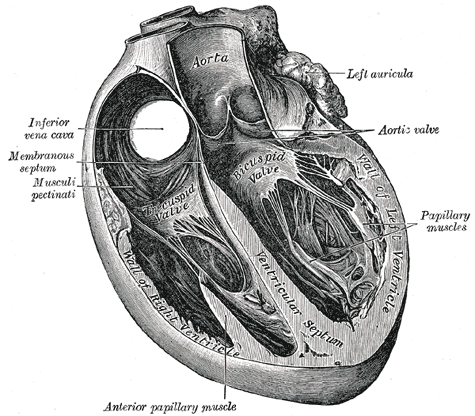
\includegraphics[width=0.7\textwidth]{figures/sample/Gray498.png} 
%\caption[Four-chamber illustration of the human heart.]{Four-chamber illustration of the human heart.  Clockwise from upper-left: right atrium, left atrium, left ventricle, right ventricle.}
%\label{fig:fourchamber}\end{figure}
The troposphere is the lowermost layer of the atmosphere ranging from the surface up to 10-15 km where the vertical temperature profile is characterized by a decrease of temperature with height.
The layer above the troposphere is called the \textit{stratosphere} where the vertical temperature gradient is reversed and temperatures increase height, this layer  and spans from   10-20 km up to 50 km in altitude \citep{andrews1987}. 
The layer in between the troposphere and the stratosphere is the tropopause, which is a transition region where the vertical temperature gradient reverses and the atmosphere is stable to upward motions. 

%The chemistry and dynamics of the stratosphere are very different from the troposphere both in temporal and spatial scales. The stratosphere is generally drier and well-mixed so that local ultraviolet absorption and infrared radiative loss exert the largest influence over the seasonal cycle of temperature and zonal winds in this layer \citep{andrews1987}.
%The strength of the inversion layer of the tropopause prevents ascending tropospheric parcels from entering the stratosphere. However, the tropopshere and stratosphere do communicate and exchange momentum and mass through waves, intrusions and radiation. 
% These exchanges typically include the tropopause. exists between stratosphere and troposphere. 

Stratosphere-troposphere coupling refers to events or processes where the two layers are notably affected by each other so that the temperature or wind flow of the two layers vary together, or \textit{couple}. One prominent example of this coupling is the effect of the stratospheric polar vortices over the zonal flow in the troposphere \citep{thompson2005,domeisen2019}. 
However, semi-periodic climatic variability in either layer can also have effects over the other layer. The dominant mode of interannual variability in the equatorial stratosphere is such an example and is introduced in the following section. 

% in the  Generally, stratospheric processes are slower and can communicate to the other latitudes of the stratosphere with more impact than tropospheric processes where friction and other processes reduce the memory of the lowermost layer. 
%Typically, the communication between the troposphere and the stratosphere occurs from the bottom layer upwards. 
%However, evidence of communication in both directions, or coupling, has been found at low latitudes and in the midlatitudes. 

\subsection{The Quasi-biennial oscillation (QBO)}

The stratospheric quasi-biennial oscillation (QBO) was discovered 60 years ago through balloon observations  that revealed that the zonal winds reverse direction in a semi-periodic way with accompanying temperature variations \citep{ebdon1960,reed1964}. The QBO has then been characterized by further observations as alternating easterly and westerly wind regimes associated with a descending zonal wind shear from up to 50 km down to 10 km, with a mean oscillatory period of 28 months \citep{baldwin2001}. 
The downward propagation of the easterly and westerly wind regimes, amplitude and the mean period have been explained by the interaction of a broad spectrum of gravity and Kelvin waves of tropospheric origin with the equatorial stratospheric zonal mean flow  \citep{baldwin2001}.

The wind variation in the middle stratosphere associated with the QBO are greater than the seasonal cycle \citep{andrews1987} and this vertical wind shear imposes a temperature signal through the thermal wind relationship, which can be expressed as: 

\begin{equation}
\frac{\partial{u}}{\partial{z}}=\frac{-R}{H \beta}\frac{\partial^2 T}{\partial y^2}, 
\end{equation}

\noindent where $\partial u / \partial z$ is the vertical shear of the zonal wind, $R$ is the ideal gas constant, $y$ is the latitude, $H$ is a scale height of the atmosphere (7-8 km) and $\beta$ is the first derivative of the Coriolis term in the meridional coordinate $y$. 

Through this thermal wind relationship a westerly shear would have warm anomalies beneath whereas an easterly shear would impose cold temperature anomalies. In turn, these temperature anomalies couple to the mean meridional circulation \citep{baldwin2001} causing an anomaly on this circulation, an effect which is often referred as the secondary circulation of the QBO \citep{plumb1982,li1995,ribera2004}. This anomalous circulation is characterized by reduced upwelling during westerly shear phases and increased upwelling during the easterly phase. These meridional circulation perturbations adiabatically warm (anomalous descent at the equator) and cool (anomalous ascent) for westerly and easterly shears, respectively, at the equator.

The combination of dynamic and thermodynamic effects ot the QBO in the equatorial stratosphere are associated with long-distance impacts across the stratosphere \citep{holton1980,lu2020} and down to the surface \citep{garfinkel2010,gray2018}. Even though the domain of the QBO is in the tropics, the better recognized effects of the QBO are in the extra tropics, particular how the direction of the zonal mean flow in the equatorial stratosphere modulates the propagation of extratropical waves and therefore also influences the wintertime stratopsheric polar vortex \citep{lu2020}, which can have profound impacts over the surface in polar and midlatitude regions.

The meridional circulation of the QBO and the associated temperature anomaly impact the height and temperature of the tropopause in the tropics \citep{baldwin2001,tegtmeier2020,tegtmeier2020b}. 
The easterly phase of the QBO (QBOE) is associated with a higher and colder tropopause in the tropics whereas the westerly phase (QBOW) is observed with lower and warmer tropical tropopause \citep{tegtmeier2020}. These variations in the tropopause characteristics, amongst other effects associated with the QBO, have been hypothesized to affect, to different extents, a range of tropical phenomena, and in particular, deep convective systems. % such as the height and temperature of the tropopause\citep{tegtmeier2020b}. 

\subsection{Tropical teleconnections of the QBO}



 The influence of the QBO on the dynamic and thermodynamic characteristics of the tropical upper-troposphere-lower stratosphere  (UTLS) region has raised interest in possible indirect effects of the QBO over tropical deep convection and clouds.
\cite{gray1984} was amongst the first to suggest an influence of the QBO over tropical systems, in particular, that Atlantic tropical cyclone activity was enhanced during QBOW compared to QBOE. 
\cite{gray1992} further argued that the anomalous vertical wind shear associated with the QBO affects the strength of convection in monsoonal and convergence zones to the extent that the vertical wind shear can modify ENSO frequency. Their results suggest that El Niño events are favoured during QBOE and  La Niña events are more frequent during QBOW.

The evidence by \cite{gray1992} has motivated further observational and modelling research on QBO tropical teleconnections; some of this research has contested Gray's results \citep[e.g.][]{chan1995,camargo2010,hansen2016tropospheric}. 
For example, \cite{giorgetta1999} was amongst the first to use a global climate model (ECHAM4) to investigate the effects of the QBO over tropical convection. \cite{giorgetta1999} focused on the the role that the QBO plays in modulating the strength of the East Asian and Indian monsoons. Their findings suggest that monsoon variability was partially modulated by the QBO, with the strongest effects associated with the QBO found for cloudiness at 100 hPa. \cite{giorgetta1999} argued that these differences could be explained by the effect of the QBO on the UTLS static stability and a consequent effect over the vertical extent of deep tropical convection. 

\begin{figure}[t!]
\centering
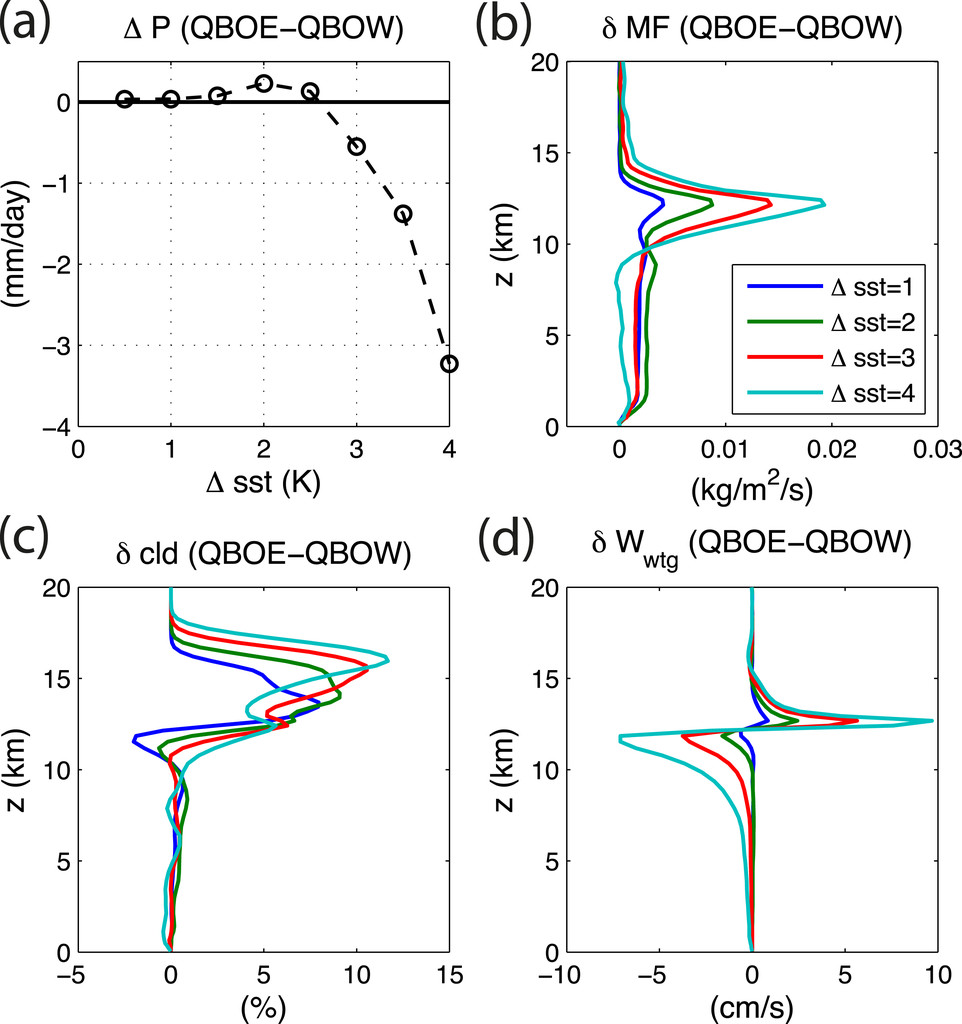
\includegraphics[width=0.85\linewidth]{figures/nie_sobel}
\caption{(a) QBO anomalous precipitation as a function of SST forcing. The $\delta sst$ are increments over a baseline of 301 K throughout the whole model domain. (b)–(d) The differences of mass flux in cloud cores, cloud fraction, and the parametrized large-scale vertical velocity derived from the weak temperature gradient approximation, respectively, between experiments with the QBOE and QBOW temperature profiles. Figure 3 from \cite{nie2015}. }
\label{fig:nie}
\end{figure}  

Further modelling work has been carried out, for instance by \cite{garfinkel2010} and \cite{garfinkel2011} that used the Whole Atmosphere Community Climate Model (WACCM) to understand the effect of the QBO over tropical precipitation, the subtropical jets and the wintertime polar vortex. \cite{garfinkel2010} shows that the canonical ENSO teleconnections to the North Pacific are stronger during QBO W in WACCM and reanalysis suggesting that the QBO modulates the wave propagation activity associated with ENSO events.

 \cite{garfinkel2011} uses perpetual winter conditions on the WACCM model and further shows that the effect of the QBO on the upper-tropospheric zonal wind in the equator and the strength and location of subtropical jets, particularly at the exit region of the jets. Their experiments show that the QBOE-QBOW zonal wind response in the upper troposphere is zonally asymmetric at the equator but zonallly symmetric in the subtropics as the subtropical jet is weakened during QBOE conditions.

 The response of convection to the QBO UTLS temperature anomalies was investigated in cloud-resolving model simulations by \cite{nie2015}. Their experimental design used the System for Atmospheric Modelling (SAM), varying SST boundary conditions with increments over a baseline SST level of 301 K, the use of the weak-temperature gradient approximation and an idealized vertical temperature profile to simulate the effect of the QBO temperature signal. 
 Figure \ref{fig:nie} shows that the precipitation and convective features differences between QBO phases depends on the SST forcing.  
 
 The precipitation difference QBOE-QBOW is positive under relatively small SST anomalies but in experiments with large SST anomalies this difference becomes negative and overall larger than under small SSTs. The difference in mass flux is also sensitive to the underlying SSTs, as increased mass flux during QBO E is increased for larger SSTs.  In other words, the QBO influence on precipitation is non monotonic and largely depends on the underlying SST field.
 
  The cloud fraction in the upper troposphere is increased during QBO E compared to QBO W whereas the ascending motions show peculiar behaviour with stronger ascent above 12 km for QBOE and weaker ascent below 12 km. 
  Their results suggest that the QBO influences convection in two ways that are non-linear and are competing mechanisms. In agreeement with previous arguments, \cite{nie2015} finds that the mas flux in the upper troposphere is increased during QBO E but also that this increases the gross moist static stability (GMS) increasing the efficiency of large-scale vertical motions during QBO E for large SSTs, which acts to reduce precipitation.  Secondly, the QBO modifies the fraction of high-level clouds resulting from deep convection which modifies the radiative heating to the column which increases precipitation during QBOE.  Figure \ref{fig:nie}a then shows how these competing effects change for different SSTs with the GMS effect dominating for large SSTs.

Various attempts have been made to determine a relationship between the QBO and deep convection in observations. 
One influential study by \cite{collimore2003} analysed satellite-derived out-going long-wave radiation (OLR) in the tropics composited by QBO phase. These composites suggest that OLR is significantly different between QBO phases in most monsoon regions, such as Central America  and the West Pacific, with an overall indication that convective activity is reduced during QBOW compared to QBOE. This influence, however, was not found to be zonally symmetric and in fact the longitudinal variations of the QBO-related OLR differences were suggestive enough that \cite{collimore2003} argued for a possible role for the QBO to modulate the Walker circulation, which would explain the lack of zonal symmetry in their results. 


Another relevant study by \cite{liess2012} found that satellite-derived cloud thickness and frequency  and upper-level velocity potential had a significant and longitudinally asymmetric response to the QBO. In particular, their results show increased convective activity during QBOE in the West Pacific but the opposite for the East Pacific.  For this reason, \cite{liess2012} also argued that the strength of the tropical overturning circulation may be modulated by the QBO, indicating the possible role of both the vertical wind shear and the upper-level static stability to modulate deep convection. 


The topic of QBO tropical teleconnections has regained attention due to recent findings suggesting a link between the QBO and the Madden-Julian Oscillation (MJO) \citep{son2017} which motivated extensive research \citep[see e.g.][]{lee2018,wang2019,martin2020jgr} due to the worldwide impact of the MJO.
 The MJO in observations shows a stronger amplitude and more predictability during QBO E, but further inspection in cloud-permitting and forecast models have not provided conclusive answers to this puzzle \citep{martin2019,martin2020jgr}. 
 
 Questions still arise as to whether this tropical link is real or due to chance, for instance \cite{wang2019} argued that the increased predictability of the MJO under the QBO E phase is included in the initial conditions, and thus not a result of a mechanistic effect of the QBO on the MJO. More generally, whether the QBO has a considerable effect on deep convection in general is debated as several plausible mechanisms exist in the literature \citep[see e.g.][]{nie2015} such as the effect of wind shear, the tropopause height, the cold-point temperature, static stability and/or feedbacks with very high cirrus and cumulunimbus clouds. 

%The use of climate models to understand these tropical teleconnections of the QBO has proven difficult due to biases in both the MJO and the QBO representations. State-of-the-art CMIP6 models struggle to reproduce several of the characteristics of the QBO \citep{richter2020}. For instance,  weaker temperature QBO signals in the lowermost tropical stratosphere in the models, e.g., compare the QBOE-W difference plot in Figure \ref{fig:qbo}. The weaker temperature signal may be key for possible biases in the tropical QBO links discussed above, such as the the QBO-MJO link which is missing from CMIP6 models \citep{kim2020} and from seasonal prediction forecast models \citep{wang2019,martin2020jgr}. 